\begin{enumerate}
	\item In an equilateral $\triangle$ ABC, D is a point on side BC such that $ BD =\frac{1}{3}BC$. Prove that $9(AD)^2 = 7(AB)^2$.
	\hfill\brak{10, 2018}\item Prove that, in a right triangle, the  square on the hypotenuse is equal to sum of the squares on the other two sides.
	\hfill\brak{10, 2018}\item Prove that the area of an equilateral triangle described on one side of the square is equal to half of the area of the equilateral triangle described on one of its diagonal.
	\hfill\brak{10, 2018}\item If the area of two similar triangles are equal, prove that they are congruent.
\hfill\brak{10, 2018}
\item In figure,\figref{fig:rightangled4} BN and CM are medians of a $\triangle$ ABC right-angled at A. Prove that \begin{align}4(BN^2 +CM^2) = 5BC^2\end{align} 
\begin{figure}[!ht]
\centering
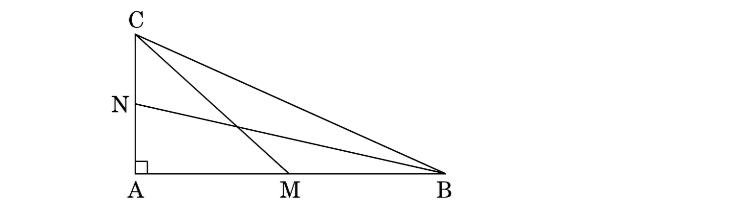
\includegraphics[width=\columnwidth]{cbse/figs/rightangled}
\caption{Right-angled triangle}
\label{fig:rightangled4}
\end{figure}

\hfill\brak{10, 2022}\item $\vec{Case Study - 1:}$
\begin{center}
$\vec{Kite Festival}$\\
\end{center}
Kite festival is celebrated in many countries at different times of the year. in India, every year 14th
January is celebrated as international kite Day. on his day many people visit India and participate in the festival by flying various kinds of kites.
\\The picture given below \figref{fig:kites5} , three kites flying together.
\begin{figure}[!ht]
\centering
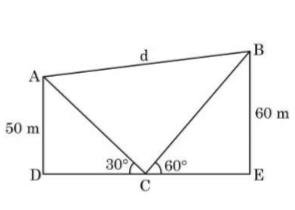
\includegraphics[width=\columnwidth]{cbse/figs/kites}
\caption{kites flying to gether}
\label{fig:kites5}
\end{figure}
\\In \figref{fig:kites5}, the angles of elevation of two kites (point C) are found to be $\degree{30}$ and  $\degree{60}$ respectively. Taking \begin{align}AD = 50 m\end{align} and\begin{align} BE = 60 m\end{align}
find
\begin{enumerate}
\item The length of string used (take them straight) for kites A and B as shown in the figure.
\item The distance 'd' between these two kites
\end{enumerate}
\hfill\brak{10, 2022}
\item Simplest form of 
 \begin{align}
     \frac{1 + \tan^{2}{A}}{1 + \cot^{2}{A}}
 \end{align}is .

\hfill\brak{10, 2020}\item Write the value of
 \begin{align}
	     \sin^{2}{30\degree} + \cos^{2}{60\degree}
	\end{align}.
\hfill\brak{10, 2020}\item If $A$, $B$ and $C$ are interior angles of $ \triangle ABC$, then show that
	\begin{align}
	    \cos \brak{\frac{B + C}{2}}=\sin \brak{\frac{A}{2}}
	\end{align}
      
\hfill\brak{10, 2020}\item Prove that : 
        \begin{align}
           (\sin^{4}{\theta} - \cos^{4}{\theta} + 1)\csc^{2}{\theta} = 2 
        \end{align}
\hfill\brak{10, 2020}
\item
If
\begin{align}
\cos\brak{\sin^{-1}{\frac{2}{\sqrt{5}}} + \cos^{-1}{x}} = 0
\end{align}
then $x$ is equal to
		\begin{multicols}{4}
\begin{enumerate}
	\item $\frac{1}{\sqrt{5}}$
	\item $-\frac{2}{\sqrt{5}}$
	\item $\frac{2}{\sqrt{5}}$
        \item $1$
\end{enumerate}
		\end{multicols}
\hfill\brak{12, 2020}
\item prove that \begin{align} \frac{\sin A-2 \sin^3A}{2\cos^3A-\cos A}=\tan A\end{align} 
  \hfill\brak{10, 2023}\item \begin{align} \sec A (1-\sin A)(\sec A+\tan A)=1\end{align} 

\hfill\brak{10, 2023}\item If 
\begin{align}
    4\cot^2 45\degree - \sec^2 60\degree + \sin^2 60\degree + p = \frac{3}{4}, 
\end{align}
then find the value of $p$.
\hfill\brak{10, 2023}\item If 
\begin{align}
    \cos A+ \cos^2A=1,
\end{align}then find the value of 
\begin{align}
\sin^2A+\sin^4A.
\end{align}
\hfill\brak{10, 2023}\item Prove that:\\
\begin{align}
\brak{\frac{1}{\cos\theta}-\cos\theta}\brak{\frac{1}{\sin\theta}-\sin\theta} = \frac{1}{\tan\theta+\cot\theta}
\end{align}




\hfill\brak{10, 2023}\item If $2\tan A=3$, then the value of $\frac{4sin A + 3\cos A}{4\sin A - 3\cos A}$ is
\begin{enumerate}
\item $\frac{7}{\sqrt{13}}$
\item $\frac{1}{\sqrt{13}}$
\item $3$
\item does not exist
\end{enumerate}



    \hfill\brak{10, 2023}\item $\brak{\sec^2\theta - 1}\brak{\csc^2\theta - 1}$  is equal to:
    \begin{enumerate}
   \item $-1$
   \item  $1$
   \item  $0$
   \item  $2$
        \end{enumerate}
   \hfill\brak{10, 2023}\item Evaluate $2\sec^2\theta+3\csc^2\theta-2\sin\theta\cos\theta$ if
   \begin{align}
      \theta=45\degree
   \end{align}
   
   \hfill\brak{10, 2023}\item If
   \begin{align}
       \sin\theta-\cos\theta=0
   \end{align}
   ,then find the value of $\sin^4\theta+\cos^4\theta$.
  \hfill\brak{10, 2023}
    \item If $\sin \theta=0$, then the value of $\tan^2\theta+\cot^2\theta$ is
    \begin{enumerate}
        \item $2$
        \item $4$
        \item $1$
        \item $\frac{10}{9}$
    \end{enumerate}
    \hfill\brak{10, 2022}\item $5\tan^2 \theta - 5\sec^2\theta = \underline{\hspace{2cm}}$
    \hfill\brak{10, 2022}\item In  \figref{fig:as.jpeg}, a tower stands vertically on the ground. From a point on the ground, which is $80m$ away from the foot of the tower, the angle of elevation of the tower is found to be $30\degree$. Find the height of the tower.
    \begin{figure}[H]
        \centering
        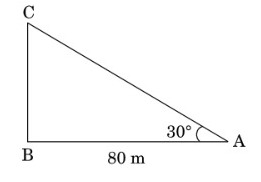
\includegraphics[width=70mm]{cbse/figs/as.jpeg}
        \caption{as.jpeg}
        \label{fig:as.jpeg}
    \end{figure}
    \hfill\brak{10, 2022}\item Show that 
    \begin{align}
        \cos(38\degree) \cos(52\degree) - \sin(38\degree)\sin(52\degree) = \cos(90\degree).
    \end{align}
    \hfill\brak{10, 2022}\item Prove that 
    \begin{align}
        \frac{\sin\theta}{\cot\theta+\csc\theta} = 2+\frac{\sin\theta}{\cot\theta-\csc\theta}.
    \end{align}
    \hfill\brak{10, 2022}\item Given 
    \begin{align}
        15 \cot (A) = 8,
    \end{align}
    find the values of $\sin (A)$ and $\sec (A)$.
    \hfill\brak{10, 2022}\item The angles of depression of the top and bottom of a tower as seen from the top of a $60\sqrt{3}m$ high cliff are $45\degree$ and $60\degree$ respectively. Find the height of the tower. (Use $\sqrt{3}=1.73$)
    \hfill\brak{10, 2022}\item The angle of elevation of the top of a building from the foot of the tower is $30\degree$ and the angle of elevation of the top of the tower from the foot of the building is $60\degree$. If the tower is $50$ meters high, then find the height of the building.
    \hfill\brak{10, 2022}\item From a point on a bridge across a river, the angles of depression of the banks on opposite sides of the river are $30\degree$ and $60\degree$ respectively. If the bridge is at a height of $3$ meters from the banks, then find the width of the river. 
    \hfill\brak{10, 2022}\item In \figref{fig:ak}, Gadisar Lake is located in the Jaisalmer district of Rajasthan. It was built by the King of Jaisalmer and rebuilt by Gadsi Singh in the $14$th century. The lake has many Chhatris. One of them is shown below:
    \begin{figure}[H]
        \centering
    	 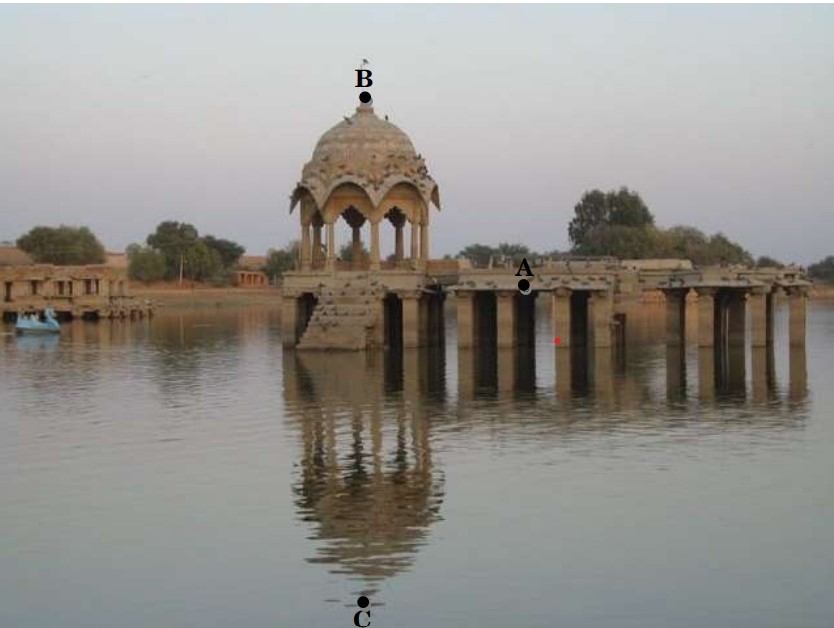
\includegraphics[width=70mm]{cbse/figs/ak.jpeg}
        \caption{ak.jpg}
        \label{fig:ak}
    \end{figure}
    Observe the picture. From a point $A$ $h$ meters above the water level, the angle of elevation of the top of Chhatri (point $B$) is $45\degree$ and the angle of depression of its reflection in the water (point $C$) is $60\degree$ . If the height of Chhatri above water level is (approximately) $10$ meters, then 
    \begin{enumerate}
        \item Draw a well-labeled figure based on the above information.
        \item Find the height ($h$) of the point $A$ above water level. (Use $\sqrt{3}=1.73$) 
    \end{enumerate}

    \hfill\brak{10, 2022}\item In \figref{fig:su.jpeg}, from a point on a bridge across a river, the angles of depression of the banks on opposite sides of the river are $30\degree$ and $45\degree$. If the bridge is at a height of $8$ meters from the banks, then find the width of the river.
    \begin{figure}[H]
        \centering
        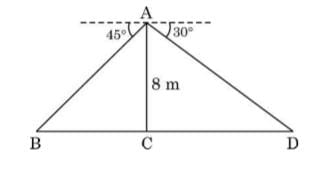
\includegraphics[width=70mm]{cbse/figs/su.jpeg}
        \caption{su.jpg}
        \label{fig:su.jpeg}
    \end{figure}
    
    \hfill\brak{10, 2022}\item Case Study-1:
    
    In \figref{fig:kite.jpeg}, Kite Festival is celebrated in many countries at different times of the year. In India, every year on $14^{th}$ January is celebrated as International Kite Day. On this day, many people visit India and participate in the festival by flying various kinds of kites.
    
    \begin{figure}[H]
	\centering
        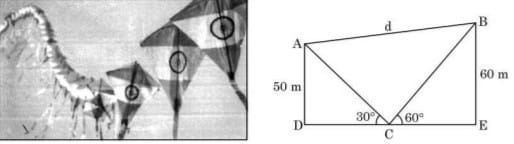
\includegraphics[width=70mm]{cbse/figs/kite.jpeg}
        \caption{kites}
        \label{fig:kite.jpeg}
    \end{figure}
    
    In Fig. 5, the angles of elevation of two kites (Point $A$ and $B$) from the hands of a man (Point $C$) are found to be $30\degree$ and $60\degree$ respectively. Taking $AD = 50$ meters and $BE = 60$ meters, find:
    \begin{enumerate}
        \item The lengths of strings used (take them straight) for kites $A$ and $B$ as shown in the figure.
        \item The distance $d$ between these two kites.
    \end{enumerate}
    
    \hfill\brak{10, 2022}\item Two boats are sailing in the sea $80$ meters apart from each other towards a cliff $AB$. The angles of depression of the boats from the top of the cliff are $30\degree$ and $45\degree$ respectively, as shown in \figref{fig:boat.jpeg}
    
    \begin{figure}[H]
        \centering
        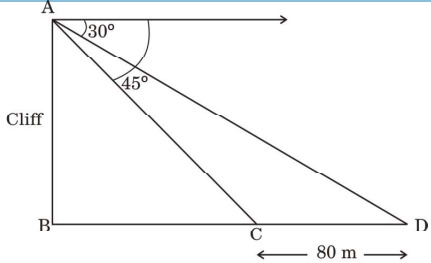
\includegraphics[width=70mm]{cbse/figs/boat.edit.jpeg}
        \caption{boat}
        \label{fig:boat.jpeg}
    \end{figure}
    
    Find the height of the cliff.
    
    \hfill\brak{10, 2022}\item The angle of elevation of the top $Q$ of a vertical tower $PQ$ from a point $X$ on the ground is $60\degree$. From a point $Y$, $40$ meters vertically above $X$, the angle of elevation of the top $Q$ of tower $PQ$ is $45\degree$. Find the height of the tower $PQ$ and the distance $PX$. (Use $\sqrt{3} = 1.73$)
    
    \hfill\brak{10, 2022}\item An Aeroplane at an altitude of $200$ meters observes the angles of depression of opposite points on the two banks of a river to be $45\degree$ and $60\degree$. Find the width of the river. (Use $\sqrt{3} = 1.732$)
    
    \hfill\brak{10, 2022}\item From the top of an $8$ meter high building, the angle of elevation of the top of a cable tower is $60\degree$ and the angle of depression of its foot is $45\degree$. Determine the height of the tower. (Take $\sqrt{3} = 1.732$).
    
    \hfill\brak{10, 2022}\item As observed from the top of a lighthouse $60$ meters high from the sea level, the angles of depression of two ships are $45\degree$ and $60\degree$. If one ship is exactly behind the other on the same side of the lighthouse, then find the distance between the two ships. (Use $\sqrt{3} = 1.732$)
    
    \hfill\brak{10, 2022}\item At a point on the level ground, the angle of elevation of the top of a vertical tower is found to be $\alpha$, such that $\tan\alpha = \frac{5}{12}$. On walking $192$ meters towards the tower, the angle of elevation $\beta$ is such that $\tan\beta = \frac{3}{4}$. Find the height of the tower.
    
    \hfill\brak{10, 2022}\item $\tan^{-1}\frac{1}{\sqrt{3}} - \cot^{-1}\frac{-1}{\sqrt{3}}$
    
    \hfill\brak{10, 2022}\item Two angles of a triangle are $\cot^{-1}2$ and $\cot^{-1}3$. The third angle of the triangle is?
    
    \hfill\brak{10, 2022}\item Solve for $x$:
    \begin{align}
        \sin^{-1}(1-x) - 2 \sin^{-1} x = \frac{\pi}{2}
    \end{align}
\hfill\brak{10, 2022}
\item If $2\cos  \theta = \sqrt{3}$ , then find the value of $\theta$
\hfill\brak{10, 2021}\item  In $\triangle ABC$, right-angled at $A$, if $AB=7 cm$ and $AC=24 cm$, then find $\sin B$
and $\tan C$.

\hfill\brak{10, 2021}\item If  $\sin (A+B) = \sqrt{3}/2,
 \sin (A-B) = 1/2,$ Where $0\degree<A+B<90\degree; A>B$, then find the values of $A$ and $B$.

\hfill\brak{10, 2021}\item  Simplify :
\begin{align}
\frac{\sin 30\degree + \tan 45\degree-\cos 60\degree}{\sec 30\degree + \cos 60\degree + \cot 45\degree} 
\end{align}


\hfill\brak{10, 2021}\item Prove that :
\begin{align}
 \sec \theta (1-\sin\theta)(\sec\theta+ \tan\theta)=1
\end{align}

\hfill\brak{10, 2021}\item Prove that :
\begin{align}
\frac{1+\sec A}{\sec A}=\frac{\sin^2 A}{1-\cos A} 
\end{align}

\hfill\brak{10, 2021}\item If  $\tan \theta = 4/3$, find the value 
$\frac{2\sin \theta -3\cos \theta}{2\sin\theta+3\cos\theta}$

\hfill\brak{10, 2021}\item If x=  $a\cos\theta$ and y=$b\sin\theta$, then find the value of   $b^2x^2+a^2y^2$

\hfill\brak{10, 2021}\item Prove that :
\begin{align}
\frac{\tan\theta-\cot\theta}{\sin\theta\cos\theta}=\tan^2\theta-\cot^2\theta 
\end{align}
\hfill\brak{10, 2021}\item Prove that:
\begin{align}
(\sec\theta-\tan\theta)^2 =\frac{1+\sin\theta}{1-\sin\theta}
\end{align}

		\hfill\brak{10, 2021}\item If $3\sin A = 1$, then find the value of $\sec A$.
		\hfill\brak{10, 2021}\item Show that: $\frac{1 + \cot^2{\theta}}{1 + \tan^2{\theta}} = \cot^2{\theta}$.
\hfill\brak{10, 2021}\item Simplify :$${\csc^{2}{60\degree} \sin^{2}{30\degree} - \sec^{2}{60\degree}}$$
	\hfill\brak{10, 2021}\item If $\tan{\theta} + \cot{\theta}$ = $\frac{4 \sqrt{3}}{3}$, then find the value of $\tan^{2}{\theta} + \cot^{2}{\theta}$. 
		\hfill\brak{10, 2021}\item Prove:$$\frac{1}{(\cot A)(\sec A) - \cot A} - \csc A = \csc A - \frac{1}{(\cot A)(\sec A) + \cot A}$$
		\hfill\brak{10, 2021}\item Prove:$$\sin^{6} A + 3\sin^{2} A \cos^{2} A = 1 - \cos^{6}  A$$
		\hfill\brak{10, 2021}\item A man on the top of a vertical tower observes a car moving at a uniform speed coming directly towards it. If it takes $18$ minutes for the angle of depression to change from $30\degree$ to $60\degree$, how soon after this will the car reach the tower ?

		\hfill\brak{10, 2021}\item A girl on a ship standing on a wooden platform, which is $50$ m above water level, observes the angle of elevation of a top of a hill as $30\degree$ and the angle of depression of the base of the hill as $60\degree$. Calculate the distance of the hill from the platform and the height of the hill.
\hfill\brak{10, 2021}
\item Two angles of a triangle are  $\cot^{-1}2$ and $\cot^{-1}3$.The third angle of the
triangle is \rule{30pt}{1pt}

\hfill\brak{12, 2021}\item Prove that $2\tan^{-1}\frac{1}{2} + \tan^{-1}\frac{1}{7} = \tan^{-1}\frac{31}{17}$

\hfill\brak{12, 2021}\item $ \sin \sbrak[\frac{\pi}{3}-\sin^{-1}(\frac{-1}{2})] $ is equal to:

\begin{enumerate}

\item $\frac{1}{2}$
\item $\frac{1}{3}$
\item -1
\item 1

\end{enumerate}

\hfill\brak{12, 2021}\item $ \sin(\tan^{-1}x)$,where $\abs{x} \le 1 $,is equal to:

\begin{enumerate}

\item$\frac{x}{\sqrt{1-x^2}}$
\item$\frac{1}{\sqrt{1-x^2}}$ 
\item$\frac{1}{\sqrt{1+x^2}}$
\item$\frac{x}{\sqrt{1+x^2}}$

\end{enumerate}  

\hfill\brak{12, 2021}\item Simplest form of $ \tan^{-1}(\frac{\sqrt{1+\cos x}+\sqrt{1-\cos x}}{\sqrt{1+\cos x}- \sqrt {1- \cos x}}) , \pi < x < \frac{3\pi}{2}$ is:

\begin{enumerate}

  \item$\frac{\pi}{4} - \frac{x}{2}$
  \item$\frac{3\pi}{2} - \frac{x}{2}$
  \item$-\frac{x}{2}$
  \item${\pi} - \frac{x}{2}$

\end{enumerate}
\hfill\brak{12, 2021}
\item Prove that 
\begin{align*}
    \sin^{-1}\frac{4}{5}+\tan^{-1}\frac{5}{12}+\cos^{-1}\frac{63}{65}=\frac{\pi}{2}
\end{align*}
\hfill\brak{12, 2019}
\item Find the value of $\sin\brak{\cos^{-1}{\frac{4}{5}}+{\tan^{-1}{\frac{2}{3}}}}$.
\hfill\brak{12, 2019}\item Solve for x:
\begin{align*}
\tan^{-1}\brak{x+1}+\tan^{-1}\brak{x-1}=\tan^{-1}\brak{\frac{8}{31}}
\end{align*}
\hfill\brak{12, 2019}\item Prove that :
\begin{align*}
\cos^{-1}\brak{\frac{12}{13}}+\sin^{-1}\brak{\frac{3}{5}}=\sin^{-1} \brak{\frac{56}{65}}
\end{align*}
\hfill\brak{12, 2019}

\item If $\tan^{-1}x-\cot^{-1}x =\tan^{-1}\brak{\frac{1}{ \sqrt3}}, x>0$ ,find the value of $x$ and hence find the value of $\sec^{-1}\left(\dfrac{2}{x}\right)$.

\hfill\brak{12, 2019}\item  If
\begin{align*}
 \sin^{-1} \brak{\dfrac{3}{x}} + \sin^{-1}\brak{\dfrac{4}{x}}=\dfrac{\pi}{2} 
\end{align*}
then find the value of $x$. 

\hfill\brak{12, 2019}\item Find the value of $x$, if $\tan \brak{\sec^{-1}\brak{\frac{1}{x}}} = \sin \brak{\tan^{-1}{2}},x > 0$.
\hfill\brak{12, 2019}

\item  Evaluate:
\begin{align*}
    \frac {\tan 65\degree}  {\cot 25\degree}
\end{align*}

\hfill\brak{10, 2019}\item Express $\brak{{\sin 67\degree}+ {\cos 75\degree}}$ in terms of trigonometric ratios of the angle between $0\degree$ and $45\degree$.

\hfill\brak{10, 2019}\item Prove that :
\begin{align*}
    \brak{\sin \theta+1+\cos \theta} \brak{\sin\theta-1+\cos\theta}.\sec\theta \csc\theta=2
\end{align*}

\hfill\brak{10, 2019}\item Prove that :
\begin{align*}
      \sqrt{\frac{\sec\theta-1}{\sec\theta+1}} + \sqrt{\frac{\sec\theta+1}{\sec\theta-1}} = 2\csc\theta
\end{align*}

\hfill\brak{10, 2019}\item If $\sec\theta + \tan\theta=m$, show that $\frac{m^2-1}{m^2+1} = \sin\theta$.

\hfill\brak{10, 2019}\item Prove that :
\begin{align*}
    2 (\sin^6\theta +\cos^6\theta) - 3 (\sin^4\theta + \cos^4\theta) + 1 = 0
\end{align*}

\hfill\brak{10, 2019}\item Find $A$ and $B$ if $\sin \brak{A + 2B}=\frac{\sqrt{3}}{2}$ and $\cos \brak{A + 4B} = 0$, where $A$ and $B$ are acute angles.





\hfill\brak{10, 2019}\item Evaluate :
 \begin{align*}
	     \sin^{2}{60\degree} + 2\tan{45\degree} - \cos^{2}{30\degree}. 
      \end{align*}

\hfill\brak{10, 2019}\item Evaluate :
\begin{align*}
\left(\frac{3\tan 41\degree}{\cot 90\degree}\right)^2 - \left(\frac{\sin 3\degree \sec 55\degree}{\tan 10\degree \tan 20\degree \tan 60\degree \tan 70\degree \tan 80\degree}\right)^2
\end{align*}

\hfill\brak{10, 2019}\item Prove that :
\begin{align*}
\frac{\tan \theta}{1-\cot \theta} + \frac{\cot \theta}{1- \tan \theta} = 1+ \sec \theta  \csc  \theta   
\end{align*}

\hfill\brak{10, 2019}\item Prove that :
\begin{align*}
    \frac{\sin \theta}{\cot \theta + \csc \theta} = 2 + \frac{\sin \theta}{\cot \theta - \csc \theta}
\end{align*}

\hfill\brak{10, 2019}\item Evaluate :
\begin{align*}
\left(\frac{3\sin 43\degree}{\cos 47\degree}\right)^2 - \frac{\cos 37\degree \csc 53\degree}{\tan 5\degree \tan 25\degree \tan 45\degree \tan 65\degree \tan 85\degree}
\end{align*}


 \hfill\brak{10, 2019}\item If $\sin A = \frac{3}{4}$, calculate $\sec A$.


\hfill\brak{10, 2019}\item If $\tan$ $\alpha$ = ${\frac {5}{12}}$, find the value of $\sec$ $\alpha$.

\hfill\brak{10, 2019}\item $A$, $B$ and $C$ are interior angles of a triangle $ABC$. Show that
\begin{enumerate}
\item  $\sin$ $ \brak{{\frac {B+C}{2}}} = \cos {\frac {A}{2}}$
\item  If $\angle A = 90 \degree$ , then find the value of $\tan \brak{{\frac{B+C}{2}}}$ 
\end{enumerate} 

\hfill\brak{10, 2019}\item If $\tan \brak{A + B} = 1$ and $\tan \brak{A - B} = \frac{1}{\sqrt{3}}$ , $0\degree$ $<$ $A + B$ $<$ $90\degree$, $A > B$, then find the values of $A$ and $B$.

\hfill\brak{10, 2019}\item If $1 + \sin^2 \theta  = 3 \sin \theta \cos \theta$, then prove that $\tan$ $\theta = 1 $ or $\tan$ $\theta = \frac{1}{2}$

\hfill\brak{10, 2019}\item Prove that :
\begin{align*}
\frac{\tan^3 \theta}{1+\tan^2 \theta} + \frac{\cot^3 \theta}{1 + \cot^2 \theta} =  \sec \theta  \csc  \theta - 2 \sin \theta \cos \theta  
\end{align*}


\hfill\brak{10, 2019}\item If $\sin{x} + \cos{y}= 1$ ; $x=30\degree$  and  $y$ is an acute angle, find the value of $y$ .

\hfill\brak{10, 2019}\item Find the value of $\cos {48\degree} - \sin {42\degree}$.

\hfill\brak{10, 2019}\item Prove that :
\begin{align*}
   {\frac{\tan\theta}{1-\tan\theta}} - {\frac{\cot\theta}{1-\cot\theta}}={\frac{\cos\theta+ \sin\theta}{\cos\theta-\sin\theta}}
\end{align*} 

\hfill\brak{10, 2019}\item If ${\cos\theta + \sin\theta} = {\sqrt 2}{\cos\theta}$, show that ${\cos\theta - \sin\theta} = {\sqrt 2}{\sin\theta}$.

\hfill\brak{10, 2019}\item Prove that :
\begin{align*}
    {\frac{(1+\cot\theta+\tan\theta)(\sin\theta-\cos\theta)}{(\sec^3\theta-\csc^3\theta)}} = \sin^2\theta \cos^2\theta
\end{align*}

\hfill\brak{10, 2019}\item Evaluate :
\begin{align*}
    {\frac{\csc^2(90\degree - \theta)-\tan^2\theta)}{2(\cos^2 37\degree + \cos^2 53\degree)}} - {\frac{2\tan^2 30\degree \sec^2 37\degree \cdot \sin^2 53\degree}{\csc^2 63\degree - \tan^2 27\degree}} 
\end{align*}	




  \hfill\brak{10, 2019}\item Prove that \begin{align*} \brak{\sin\theta + \csc\theta}^2 + \brak{\cos\theta + \sec\theta}^2 = 7 + \tan^2\theta + \cot^2\theta\end{align*}.
  \hfill\brak{10, 2019}\item Prove that \begin{align*}\brak{1+\cot A - \csc A} \brak{1 + \tan A +\sec A} = 2 \end{align*}.
  \hfill\brak{10, 2019}\item Prove that \begin{align*} \frac{\sin A-\cos A+1}{\sin A+ \cos A-1} =\frac{1}{\sec A-\tan A}\end{align*}
  \hfill\brak{10, 2019}\item Find $A$ if \begin{align*}\tan 2A = \cot (A-24\degree)\end{align*}
  \hfill\brak{10, 2019}\item Find the value of \begin{align*}(\sin^2 33\degree+ \sin^2 57\degree)\end{align*}
  
  
  \hfill\brak{10, 2019}\item if If $\sec\theta = x + \frac{1}{4x}$, where $x \neq 0$, find $(\sec\theta + \tan\theta)$.
  \hfill\brak{10, 2019}\item prove that \begin{align*} \frac{\tan^2A}{\tan^2 A-1}+\frac{\csc^2 A}{\sec^2 A-\csc^2 A}=\frac{1}{1-2\cos^2 A}\end{align*}
\hfill\brak{10, 2019}
\item If $4$ $\tan\theta=3$, evaluate \begin{align*}\brak {\frac{4 \sin\theta - \cos\theta + 1 }{ 4 \sin\theta + \cos\theta - 1 } } \end{align*}   

\hfill\brak{10, 2018}\item If $\tan2A = \cot(A-18\degree)$, where $2A$ is an acute angle, find the value of $A$.

\hfill\brak{10, 2018}\item What is the value of $ \brak{\cos^2 67\degree - \sin^2 23\degree}$ ?

\hfill\brak{10, 2018}\item  Prove that:$\brak{\frac{\sin A - 2sin^3 A}{2 \cos^3 A-\cos A} = \tan A }$

			\hfill\brak{10, 2018}
\item Find the value of
	\begin{align*}
		\tan^{-1}\sqrt{3}-\cot^{-1}\brak{\sqrt{-3}}
	\end{align*}
 \hfill\brak{12, 2018}\item Prove that 
			\begin{align*}
		3\sin^{-1}x=\sin^{-1}\brak{3x-4x^3}, x\in\brak{\frac{-1}{2},\frac{1}{2}}
			\end{align*} 

\hfill\brak{12, 2018}\item Prove that :
	\begin{align*}
		\cos^{-1}\brak{\frac{12}{13}}+\sin^{-1}\brak{\frac{3}{5}}=\sin^{-1} \brak{\frac{56}{65}}
	\end{align*}
 \hfill\brak{12, 2018}\item Prove that :
         \begin{align}
          \sin^{-1}\brak{\dfrac{8}{17}}+\cos^{-1}\brak{\dfrac{4}{5}}=\cot^{-1}\brak{\dfrac{36}{77}}
         \end{align}

\hfill\brak{12, 2018}\item Prove that :
    \begin{align*}
       \sin^{-1}\dfrac{4}{5}+\tan^{-1}\dfrac{5}{12}+\cos^{-1}\dfrac{63}{65}=\dfrac{\pi}{2}
    \end{align*}

\hfill\brak{12, 2018}\item If $\tan^{-1}{x} - \cot^{-1} {x}= tan^{-1}\brak{\frac{1}{\sqrt{3}}},$ $x > 0,$ find the value of $x$ and hence find the value of $\sec^{-1}\brak{\frac{2}{x}}$.
 \hfill\brak{12, 2018}\item If $\sin^{-1}\brak{\frac{3}{x}} + \sin^{-1}\brak{\frac{4}{x}} = \frac{\pi}{2}$, then find the value of $x$.
 \hfill\brak{12, 2018}\item Find  the value of $x$, if $\tan\brak{\sec^{-1}\brak{\dfrac{1}{x}}}  = \sin \brak{\tan^{-1}{2}},x>0$.

\hfill\brak{12, 2018}
\item Find the value of $\sin\brak{\cos^{-1}{\frac{4}{5}}+{\tan^{-1}{\frac{2}{3}}}}$
\hfill\brak{12, 2018}\item Solve for $x$:
	\begin{align*}
	\tan^{-1}\brak{x+1}+\tan^{-1}\brak{x-1}=\tan^{-1}\brak{\dfrac{8}{31}}
	\end{align*}
\hfill\brak{12, 2018}
\item Solve : $\tan^{-1}4x+\tan^{-1}6x=\frac{\pi}{4}$
\hfill\brak{12, 2018}
\item Solve for x :  $\tan^{-1}(2x)+\tan^{-1}(3x)=\frac{\pi}{4}$
\hfill\brak{12, 2018}

\item if $\tan^{-1}\dfrac{x-3}{x-4} + \tan^{-1}\dfrac{x+3}{x+4} =\dfrac{\pi}{4}$, then find the value of $x$ .
\hfill\brak{12, 2017}

	\item Prove that $ 2\sin^{-1} \brak{\frac{3}{5}} - \tan^{-1} \brak{\frac{17}{31}} = \frac{\pi}{4}$

	\hfill\brak{12, 2016}\item Solve the equation for $x$: $\cos (\tan^{-1}) = \sin \brak{\cot^{-1} \frac{3}{4}} = \sin \brak{\cot^{-1} \frac{3}{4}}$

	
	\hfill\brak{12, 2016}\item Solve for 
	\begin{align*}
		x: \tan^{-1}(x-1) + \tan^{-1}x + \tan^{-1}(x+1) = \tan^{-1}3x
	\end{align*}

	\hfill\brak{12, 2016}\item Prove that 
	\begin{align*}
	\tan^{-1} \brak{\frac{6x-8x^{3}}{1-12x^{2}}} - \tan^{-1} \brak{\frac{4x}{1-4x^{2}}} = \tan^{-1}2x;
	\end{align*}
	\begin{align*}
		\abs{2x} < \frac{1}{\sqrt{3}}
	\end{align*}

 	\hfill\brak{12, 2016}\item Prove that 
	\begin{align*}
		2\sin^{-1}\brak{\frac{3}{5}}-\tan^{-1}\brak{\frac{17}{31}} = \frac{\pi}{4}
	\end{align*}
	\hfill\brak{12, 2016}\item Solve the equation for x:
	\begin{align*}
	\cos\brak{\tan^{-1}x} = \sin\brak{\cot^{-1}\frac{3}{4}}
	\end{align*}
\hfill\brak{12, 2016}
\item Prove that $2\tan^{-1}\brak{\frac{1}{2}}+\tan^{-1}\brak{\frac{1}{7}} = \sin^{-1}\brak{\frac{31}{25\sqrt{2}}}$. 

\hfill\brak{12, 2015}\item Solve for x: $\tan^{-1}\brak{\frac{1-x}{1+x}} = \frac{1}{2}\tan^{-1}x$, $x>0$. 
\hfill\brak{12, 2015}
\item The length of the shadow of a tower on the plane ground is $\sqrt{3}$ times the height of the tower.Find the angle of elevation of the sun.

\hfill\brak{10, 2023}\item  The angle of elevation of the top of a tower from a point on the ground which is $30$ m away from the foot of the tower,is $30\degree$ .Find the height of the tower.

\hfill\brak{10, 2023}\item  As observed from the top of a $75$ m high lighthouse from the sea-level,the angles of depression of two ships are $30\degree$ and $60\degree$.If one ship is exactly behind the other on the same side of the lighthouse,find the distance between two ships.$\brak{Use \sqrt{3} = 1.73}$

\hfill\brak{10, 2023}\item  From a point on the ground,the angle of elevation of the bottom and top of a transmission tower fixed at the top of $30$ m high building are $30\degree$ and $60\degree$, respectively.Find the height of the transmission tower.$\brak{Use \sqrt{3} = 1.73}$
 \hfill\brak{10, 2023}   

\item A straight highway leads to the foot of a tower.A man standing on the top of the $75$ m high tower observes two cars at angles of depression of $30\degree$ and $60\degree$,Which are approaching the foot of the tower.If one car is exactly behind the other on the same side of the tower,find the distance between the two cars.
    \hfill\brak{10, 2023}\item From the top of a $7$ m high building, the angle of elevation of the top of a cable tower is $60\degree$ and the angle of depression of its foot is $30\degree$.Determine the height of the tower.(take $\sqrt{3}=1.73$)
\hfill\brak{10, 2023}\item The angle of elevation of the top of a tower $24$ m high from the foot of another tower in the same plane is ${60}{\degree}$. The angle of elevation of the top of second tower from the foot of the first tower is ${30}{\degree}$. Find the distance between two towers and the height of the other tower. Also, find the length of the wire attached to the tops of both the towers.
\hfill\brak{10, 2023}\item A spherical balloon of radius $r$ subtends an angle of ${60}{\degree}$ at the eye of an observer. If the angle of elevation of its centre is ${45}{\degree}$ from the same point, then prove that height of the centre of the balloon is $\sqrt{2}$ times its radius.
    \hfill\brak{10, 2023}

\item A vertical pole is $100$ metres high. Find the angle subtended by the pole at a point on
the ground $100 \sqrt{3}$ meters from the base of the pole.

    \hfill\brak{10, 2021}\item The angle of elevation of the top of a tower from a point is found to be $60\degree$.At a point $40$ m above the first point, the angle of elevation of the top of the tower is $45\degree$.Find the height of the tower.
    \hfill\brak{10, 2021}\item A statue $1.6$m tall stands on the top of a pedestal. From a point on the ground, the angle of elevation of the top of statue is $60\degree$ and from the same point, the angle of elevation of the top of the pedestal is $45\degree$.Find the height of the pedestal.
    \hfill\brak{10, 2021}\item Two poles, $6$m and $11$ m high, stand vertically on the ground. If the distance between their feet is $12$ m, find the distance between their tops.

	\hfill\brak{10, 2021}\item The angle of elevation of the top of a tower from a point on the ground,which is $30$ m away from the foot of the tower is $45\degree$ .What is the height of the tower ?
	\hfill\brak{10, 2021}\item Find the sun's altitude if the shadow of a 15 m high tower is ${15}\sqrt{3}$ m.
	\hfill\brak{10, 2021}\item From a point on the ground, $20$ m away from the foot of vertical tower, the angle of elevation of the top of the tower is $60\degree$. Find the height of the tower.
			\hfill\brak{10, 2021}\item In $\triangle$ $ABC$, $AB = {4\sqrt{3}}$ cm, $AC = 8 cm$ and $BC = 4 cm$. The angle $B$ is
				\begin{enumerate}
\item $120\degree$
\item $90\degree$
\item $60\degree$
\item $45\degree$
				\end{enumerate}
	\hfill\brak{10, 2021}\item To explain how trignometry can be used measure the height of an inaccessible object, a teacher gave the following example to students :

		A TV tower stands vertically n the bank of a canal. From a point on the other bank direct opposite the tower, the angle of the elevation of the top of the tower is $60\degree$.From another point 20 m away from this point to the foot of the tower, the angle of elevation of the top of the tower is $30\degree$ (as shown in Figure 1).

		\begin{figure}[H]
			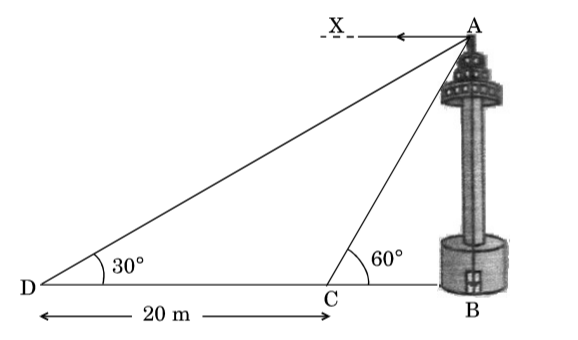
\includegraphics[width=0.75\columnwidth]{cbse/figs/Problem.png}
			\caption{Projection of Tower}
			\label{fig:traingle}
		\end{figure}
		Based on the above, answer the following questions :
		\begin{enumerate}
			\item The width of the canal is
				\begin{enumerate}
					\item ${10}\sqrt{3} m$
					\item ${20}\sqrt{3} m$
					\item $10 m$
					\item $20 m$
				\end{enumerate}
			\item Height of the tower is
				\begin{enumerate}
					\item ${10}\sqrt{3} m$
					\item $10 m$
					\item ${20}\sqrt{3} m$
					\item $20 m$
				\end{enumerate}
			\item Distance of the foot of the tower from the point $D$ is
				\begin{enumerate}
					\item $20 m$
					\item $30 m$
					\item $10 m$
					\item ${20}\sqrt{3} m$
				\end{enumerate}
\end{enumerate}
\hfill\brak{10, 2021}
\item In \figref{fig:Fig-4.png}, the angle of elevation of the top of a tower from a point $C$ on the ground, which is $30m$ away from the foot of the tower, is $30\degree$. Find the height of the tower.      
\begin{figure}[H]
\centering
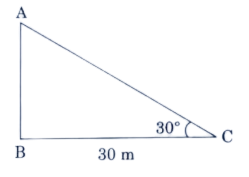
\includegraphics[width=0.75\columnwidth]{cbse/figs/Fig-4.png}
\caption{}      
\label{fig:Fig-4.png}
\end{figure}
\hfill\brak{10, 2020}\item A statue $1.6m$ tall, stands on the top of a pedestal. From a point on the ground, the angle of elevation of the top of the statue is $60\degree$ and from the same point the angle of elevation of the top of the pedestal is $45\degree$. Find the height of the pedestal.(Use $\sqrt{3}=1.73$)
\hfill\brak{10, 2020}
\item A moving boat is observed from the top of a $150m$ high cliff moving away from the cliff. The angle of depression of the boat changes from $60\degree$ to $45\degree$ in $2$ minutes. Find the speed of the boat in m/min.

\hfill\brak{10, 2019}\item There are two poles, one each on either bank of a river just opposite to each other. One pole is $60m$ high. From the top of this pole, the angle of depression of the top and foot of the other pole are $30\degree$ and $60\degree$respectively. Find the width of the river and height of the other pole.

\hfill\brak{10, 2019}\item Two poles of equal heights are standing opposite to each other on either side of the road which is $80 m$ wide. From a point $P$ between them on the road, the angle of elevation of the top of a pole is $60\degree$ and the angle of depression from the top of the other pole of point $P$ is $30\degree$. Find the heights of the poles and the distance of the point $P$ from the poles.

\hfill\brak{10, 2019}\item Amit, standing on a horizontal plane, finds a bird flying at a distance of $200 m$ from him at an elevation of $30\degree$. Deepak standing on the roof of a $50 m$ high building, finds the angle of elevation of the same bird to be $45\degree$. Amit and Deepak are on opposite sides of the bird. Find the distance of the bird from Deepak.

\hfill\brak{10, 2019}\item From a point $P$ on the ground, the angle of elevation of the top of a tower is $30\degree$ and that of the top of the flag-staff fixed on the top of the tower is $\sqrt{5}$. If the length of the flag-staff is $5 m$, find the height of the tower. (Use $\sqrt{3}= 1.732$).


\hfill\brak{10, 2019}\item The shadow of a tower standing on a level ground is found to be $40 m$ longer when the Sun's altitude is $30\degree$ than when it was $60\degree$. Find the height of the tower. $(Given \sqrt{3} = 1.732)$

\hfill\brak{10, 2019}\item A man in a boat rowing away from a light house $100m$  high takes $2$ minutes to change the angle of elevation of the top of the light house from $60\degree$ to $30\degree$. Find the speed of the boat in metres per minute. [Use $\sqrt{3}=1.732$]
\hfill\brak{10, 2019}\item Two poles of equal heights are standing opposite each other on either side of the road, which is $80 m$  wide. From a point between them on the road, the angles of elevation of the top of the poles are $60\degree$ to $30\degree$ respectively. Find the height of the poles and the distances of the point from the poles.
\hfill\brak{10, 2019}
		\item As observed from the top of a $100 m$ high light house from the sea level, the angles of depression of two ships are $30\degree$ and $45\degree$. If one ship is exactly behind the other on the same side of the light house, find the distance between the two ships. ({\textbf{Use}} $\sqrt3 = 1.732$)
\hfill\brak{10, 2018}
\item A statue, $1.46$m tall, stands on a pedestal. From a point on the ground the angle of elevation of the top of the statue is $60\degree{}$ and from the same point angle of elevation of the top of the pedestal is $45\degree{}$. Find the height of the pedestal. $\brak{use \sqrt{3}=1.73}$
\hfill\brak{10, 2018}
\item A ladder, leaning against a wall, makes an angle of $60 \degree$ with the horizontal.If the foot of the ladder is $2.5$ m away from the wall, find the length of the ladder.\\
\hfill\brak{10, 2016}\item  A man standing on the deck of a ship, which is $10$ m above water level, observes the angle of elevation of the top of a hill as $ 60\degree $ and the angle of depression of the base of hill as $ 30 \degree $. Find the distance of the hill from the ship and the height of the hill.\\
\hfill\brak{10, 2016}\item The angle of elevation of the top $Q$ of a vertical tower $PQ$ from a point $X$ on the ground is $ 60\degree $. From a point $Y$, $40$ m vertically above $X$, the angle of elevation of the top $Q$ of tower is $ 45 \degree $. Find the height of the tower $PQ$ and the distance $PX$. $\brak{\text{Use }\sqrt{3} = 1.73}$\\
\hfill\brak{10, 2016}
\item A boy standing on a horizontal plane finds a bird flying at a distance of $100 m$ from him at an elevation of $30\degree$. A girl standing on the roof of a $20 m$ high building, finds the elevation of the same bird to be $45\degree$. The boy and the girl are on the opposite sides of the bird. Find the distance of the bird from the girl. (Given ${\sqrt 2}= 1.414$)

\hfill\brak{10, 2019}\item The angle of elevation of an aeroplane from a point $A$ on the ground is $60\degree$. After a flight of $30 $seconds , the angle of elevation changes to $30\degree$. If the plane is flying at a constant height of $3600\sqrt 3 $ metres, find the speed of the aeroplane.

\hfill\brak{10, 2019}
\item If $\sin\theta+\cos\theta=\sqrt{2}\cos\brak{90\degree{}-\theta}$, find the value of $\cot\theta$.
\hfill\brak{10, 2018}\item Prove that : $\dfrac{1}{\cosec\theta+\cot\theta}-\dfrac{1}{\sin\theta}=\dfrac{1}{\sin\theta}-\dfrac{1}{\cosec\theta-\cot\theta}$
\hfill\brak{10, 2018}\item If $\tan\theta+\sin\theta=m$, $\tan\theta-\sin\theta=n$, show that $m^{2}-n^{2}=4\sqrt{mn}$
\hfill\brak{10, 2018}\item Prove that : $\brak{\dfrac{\sin A}{1-\cos A}-\dfrac{1-\cos A}{\sin A}}.\brak{\dfrac{\cos A}{1-\sin A}-\dfrac{1-\sin A}{\cos A}}=4$.
\hfill\brak{10, 2018}
\item If a tower $30$ m high, casts a shadow $10\sqrt{3}$ m long on a ground, then what is the angle of elevation of the sun ?
\hfill\brak{10, 2017}\item A man observes a car from the top of a tower, which is  moving towards the tower with a uniform speed. If the angle of depression of the car changes from $30\degree$ to $45\degree$ in $12$ minutes, find the time taken by the car now to reach the tower.
\hfill\brak{10, 2017}\item An aeroplane is flying at a height of $300 m$ above the ground. Flying at this height, the angles of depression from the aeroplane of two points on both banks of a river in opposite directions are $45\degree$ and $60\degree$ respectively. Find the width of the river. 
\hfill $\sbrak{Use \sqrt 3 = 1.732}$
\hfill\brak{10, 2017}\item On a straight line passing through the foot of a tower, two points $C$$D$ are at distances of $4$ m
and $16$ m from the foot respectively. If the angles of elevation from$C$$D$ of the top tower are complementary, then find the height of the tower.  
\hfill\brak{10, 2017}\item From the top of a tower, $100$ m high, a man observes two cars on the opposite sides of the tower and in same straight line with its base, with angles of depression $30\degree$ and $45\degree$. Find the distance between the cars.
\hfill  $\sbrak{Take \sqrt{3} = 1.732}$
\hfill\brak{10, 2017}

\item Solve for $x$: $\tan^{-1}(x-1) + \tan^{-1}x + \tan^{-1}(x+1) = \tan^{-1}3x$.
\hfill\brak{12, 2016}\item Prove that $\tan[\frac{6x-8x^3}{1-12x^2}]-\tan^{-1}[\frac{4x}{1-4x^2}]=\tan^{-1}2x:|2x|<\frac{1}{\sqrt{3}}$
\hfill\brak{12, 2016}\item Solve for x: $tan^{-1}(\frac{2-x}{2+x}) = \frac{1}{2} tan^{-1}\frac{x}{2},x>0$
\hfill\brak{12, 2016}
\item At a point $A$, $20$ metres above the level of water in a lake, the angle of elevation of a cloud is $30 \degree.$ The angle of depression of the reflection of the cloud in the lake, at $A$ is $60\degree .$ Find the distance of the cloud from $A$.
\hfill\brak{10, 2015}\item In Figure \ref{Figure 1}, a tower $AB$ is $20$ m high and $BC$, its shadow on the ground,is $20\sqrt{3}$ m long. Find the sun's altitude.
\begin{figure}[h!]
	\centering
    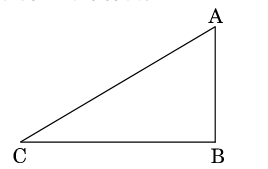
\includegraphics[width=\columnwidth]{cbse/figs/cbse_30_3_1.png}
	\caption{}
	\label{Figure 1}
\end{figure}
\hfill\brak{10, 2015}\item The angle of elevation of an aeroplane from a point $A$ on the ground is $60 \degree  $. After a flight of $15$ seconds, the angle of elevation changes to $  30 \degree.$ If the aeroplane is flying at a constant height of $1500\sqrt{3}$ m, find the speed of the plane in km/hr.
\hfill\brak{10, 2015}
\item A kite is flying at a height of $30 \text{ m}$ from the ground. The length of string from the kite to the ground is $60 \text{ m}$. Assuming that there is no slack in the string, the angle of elevation of the kite at the ground is 
\hfill\brak{10, 2012}\item From a point on the ground, which is $15\text{ m}$ away from the foot of a vertical tower, the angle of elevation of the top of the tower, is found to be $60\degree$. The height of the tower in $\brak{\text{in metres}}$ is 
\hfill\brak{10, 2012}\item The length of shadow of a tower on the plane ground is $\sqrt 3 \text{ m}$ times the height of the tower. The angle of elevation of sun is : 
\hfill\brak{10, 2012}\item The angles of depression of the top and bottom of a tower as seen from the top of a $60\sqrt 3 \text{ m}$ high cliff are $45\degree$ and $60\degree$ respectively. Find the height of the tower. 
%Trigonometry
\hfill\brak{10, 2012}\item In a flight of $2800 \text{ km}$, an aircraft was slowed down due to bad weather. Its average speed is reduced by $100 \text{ km/h}$ and time is increased by $30$ minutes. Find the original duration of flight. 
%Trigonometry
\hfill\brak{10, 2012}\item The angles of elevation and depression of the top and bottom of a light-house from the top of a $60 \text{ m}$ high building are $30\degree$ and $60\degree$ respectively. Find 
\begin{enumerate}
\item the difference between the heights of the light-house and the building. 
\item the distance between light-house and building. 
\end{enumerate}
%trigonometry
\hfill\brak{10, 2012}\item The angles of depression of two ships from the top of a light house and on the same side of it are found to be $45\degree$ and $30\degree$. if the ships are $200 \text{ km}$ apart, find the height of the light house. 
\hfill\brak{10, 2012}\item The angle of elevation of the top of a hill at the foot of a tower is $60\degree$ and the angle of depression from the top of the tower of the foot of the hill is $30\degree$. If the tower is $50\text{ m}$ high, find the height of the hill. 
\hfill\brak{10, 2012}\item From the top of a tower $50\text{ m}$ high, the angle of depression of the top of a pole is $45\degree$ and from the foot of the pole, the angle of elevation of the top of the tower is $60\degree$. find the height of the pole if the pole and tower stand on the same plane. 
\hfill\brak{10, 2012}\item The angle of depression from the top of a tower of a point $A$ on the ground is $30\degree$. On moving a distance of $20\text{ m}$ from the point $A$ towards the foot of the tower to a point $B$ the angle of elevation of the top of the tower from point $B$ is $60\degree$. Find the height of the tower and its distance from point $A$.
\hfill\brak{10, 2012}
\item A tower stands vertically on the ground. From a point on the ground which is $25$ m away from the foot of the tower, the angle of elevation of the top of the tower is found to be $45\degree$. Then the height $\brak{in\,meters}$ of the tower is



\hfill\brak{10, 2011}\item The angle of elevation of the top of a vertical tower from a point on the ground is $60\degree$. From another point $10$ m vertically above the first, its angle of elevation is $30\degree$. Find the height of the tower.


\hfill\brak{10, 2011}\item From the top of a vertical tower, the angles of depression of two cars, in the same straight line with the base of the tower, at an instant are found to be $45\degree$ and $60\degree$. If the cars are $100$ m apart and are on the same side of the tower, find the height of the tower. 

[Use $\sqrt{3} = 1.73$]
\hfill\brak{10, 2011}
    \item The angle of elevation of the top of a tower from a point on the ground, which is 30 m away from the foot of the tower is 45°. The height of the tower (in metres) is
    \hfill\brak{10, 2011}\item From the top of a tower $100$ $m$ high, a man observes two cars on the opposite sides of the tower with angles of depression $30^\circ$ and $45^\circ$ respectively. Find the distance between the cars. [Use $\sqrt{3}=1.73$].
    \hfill\brak{10, 2011}\item Two poles of equal heights are standing opposite to each other on either side of the road, which is $100m$ wide. From a point between them on the road, the angles of elevation of the top of the poles are $60^\circ$ and $30^\circ$, respectively. Find the height of the poles.
\hfill\brak{10, 2011}


\item Write the principal value of $\sec^{-1} \brak{-2}$.

\hfill\brak{12, 2010}\item Prove the following:
    \begin{align*}
        \cos \sbrak{\tan^{-1} \cbrak{\sin \brak{cot^{-1} x}}} = \sqrt{\frac{1 + x^2}{2 + x^2}}
    \end{align*}

\hfill\brak{12, 2010}\item Prove the following:
    \begin{align*}
        \tan^{-1} x + \tan^{-1} \brak{\frac{2x}{1 - x^2}} = \tan^{-1} \brak{\frac{3x - x^3}{1 - 3x^2}}
    \end{align*}
\hfill\brak{12, 2010}
\item A man standing on the deck of a ship, which is 10 m above the water level, observes the
angle of elevation of the top of a hill as 60° and the angle of depression of the base of the hill as
300. Calculate the distance of the hill from the ship and the height of the hill.

\hfill\brak{10, 2006}\item From a window $x$ meters high above the ground in a street, the angles of elevation and depression of the top and foot of the other house on the opposite side of the street are $\alpha$ and $\beta$ respectively. Show that the height of the opposite house is $x(1 + \tan \alpha \cot \beta)$ meters.

\hfill\brak{10, 2006}
\item Find the value of $\tan^{-1} (-\frac{1}{\sqrt{3}}) + \cot^{-1}(\frac{1}{\sqrt{3}}) + \tan^{-1}[\sin(-\frac{\pi}{2})]$
	 \hfill\brak{10, 2024}
\item If $\sec\theta - \tan\theta = m$, then the value of $\sec\theta + \tan\theta$ is:

 \hfill\brak{10, 2024}\item If $\cos(\alpha + \beta) = 0$ then the value of $\cos\left(\frac{\alpha + \beta}{2}\right)$ is equal to:
hfill\brak{10, 2024}

\item Simplify: $\cos^{-1}x + \cos^{-1}\sbrak{\frac{x}{2}{\frac{\sqrt{3-3x^2}}{2}}};-\frac{1}{2} \leq x \leq 1$

\hfill\brak{12, 2024}\item\textbf{ Evaluate:} $2\sqrt{2} \cos 45\degree \sin 10\degree + 2\sqrt{3} \cos 30\degree$

\hfill\brak{10, 2024}\item If  $A = 60\degree$ and  $B = 30\degree$, verify that : $\sin\brak{A + B} = \sin A \cos B + \cos A \sin B$

\hfill\brak{10, 2024}\item Prove that : $\frac{\tan{\theta}}{1 - \cot{\theta}} + \frac{\cot{\theta}}{1 - \tan{\theta}} = 1 + \sec
{\theta}\csc{\theta}$
\hfill\brak{10, 2024}\item A pole $6m$ high is fixed on the top of a tower. The angle of elevation of the top of the pole observe
d from a point $P$ on the ground is $60\degree$ and the angle of depression of the point $P$ from the top of
 the tower is $45\degree$. Find the height of the tower and the distance of point $P$ from the foot of the t
ower
\hfill\brak{10, 2024}

\item If $ a = \sin^{-1}\left(\frac{\sqrt{2}}{2}\right) + \cos^{-1}\left(\frac{-1}{2}\right) $ and $ b = \tan^{-1}(\sqrt{3}) + \cot^{-1}\left(\frac{-1}{\sqrt{3}}\right) $, then find the value of $a + b$.





\hfill\brak{12, 2024}\item Find the value k if 
\\ 
	\begin {align}
	\sin^{-1} \left[k \tan \left( 2\cos^{-1} \frac {\sqrt{3}}{2}\right)\right]= \frac{\pi}{3}.
\end {align}
\hfill\brak{12, 2024}

\item If $4 \cot^{2}45\degree-\sec^{2}60\degree+\sin^{2}60\degree+p=\frac{3}{4},$ then find the value of p.

\hfill\brak{10, 2023}\item If $\cos A$ + $\cos^{2}A = 1$ ,then find the value of $\sin^{2}A$ + $\sin^{4}A$

\hfill\brak{10, 2023}\item The length of the shadow of a tower on the plane ground is $ \sqrt3 $ times the height of the tower. Find the angle of elevation of the sun.

\hfill\brak{10, 2023}\item The angle of elevation of the top of a tower from a point on the ground which is $30 \mathrm{m}$ away from the foot of the tower,is $30\degree$.Find the height of the tower.

\hfill\brak{10, 2023}\item Prove that :
\begin{align}
	\brak{\frac{1}{\cos\theta}-\cos\theta} \brak{\frac{1}{\sin\theta}-\sin\theta} = \frac{1}{\tan\theta + \cot\theta}
\end{align}

\hfill\brak{10, 2023}\item As observed from the top of a $75 \mathrm{m}$ high lighthouse from the sea-level, the angles of depression of two ships are $30\degree$ and $60\degree$. If one ship is exactly behind the other on the same side of the lighthouse, find the distance between the two ships.\\
	$\brak{Use \sqrt{3} = 1.73}$

\hfill\brak{10, 2023}\item From a point on the ground, the angle of elevation of the bottom and top of a transmission tower fixed at the top of $30 \mathrm{m}$ high building are $30\degree$ and $60\degree$, respectively. Find the height of the transmission tower. $\brak{Use\sqrt{3} = 1.73}$.
	\hfill\brak{10, 2023}\item If a pole 6 m high casts a shadow $2 \times \sqrt{3}$m long on the ground,then sun's elevation is:
	\begin{enumerate}
\item $60\degree$
\item $45\degree$
\item $30\degree$
\item $90\degree$
	\end{enumerate}
 \hfill\brak{10, 2023}\item $ (\sec^2 \theta - 1)(\cosec^2 \theta - 1)$
is equal to:
\begin{enumerate}
\item $-1$
\item $1$
\item $0$
\item $2$
\end{enumerate}

\hfill\brak{10, 2023}\item
Evaluate \begin{align}
2\sec^2\theta + 3\csc^2\theta - 2\sin\theta\cos\theta  \ \text{if} \ \theta = 45\degree.
\end{align}
\hfill\brak{10, 2023}\item 
If \begin{align} 
\sin\theta - \cos\theta = 0, \text{ then find the value of }\sin^4\theta + \cos^4\theta.
\end{align}
\hfill\brak{10, 2023}\item
Prove that \begin{align} \frac{\sin{A}-2sin^3{A}}{2\cos^3{A}-\cos{A}}=\tan{A} \end{align}
\hfill\brak{10, 2023}\item
Prove that \begin{align} \sec{A\brak{1-\sin{A}}\brak{\sec{A}+\tan{A}}}=1. \end{align}
\hfill\brak{10, 2023}\item
	A straight highway leads to the foot of a tower. A man standing on the top of the $75 \mathrm{m}$ high tower observes two cars at angles of depression of $30^\circ$ and $60^\circ$, which are approaching the foot of the tower. If one car is exactky behind the other on the same side of the tower, fin
d the dist
ance between the two cars. use \brak{\sqrt{3}=1.73}.
\hfill\brak{10, 2023}\item
	From the top of a $7 \mathrm{m}$ building, the angle of elevation of the top a cable tower is 60\degree and the angle of depression of its foot is 30\degree. Determine the height of the tower.

\hfill\brak{10, 2023}

\end{enumerate}
